% !TEX TS-program = pdflatex
% !TEX encoding = UTF-8 Unicode

% This is a simple template for a LaTeX document using the "article" class.
% See "book", "report", "letter" for other types of document.

\documentclass[11pt]{article} % use larger type; default would be 10pt

\usepackage[utf8]{inputenc} % set input encoding (not needed with XeLaTeX)

%%% Examples of Article customizations
% These packages are optional, depending whether you want the features they provide.
% See the LaTeX Companion or other references for full information.

%%% PAGE DIMENSIONS
\usepackage{geometry} % to change the page dimensions
\geometry{a4paper} % or letterpaper (US) or a5paper or....
% \geometry{margin=2in} % for example, change the margins to 2 inches all round
% \geometry{landscape} % set up the page for landscape
%   read geometry.pdf for detailed page layout information

\usepackage{graphicx} % support the \includegraphics command and options

% \usepackage[parfill]{parskip} % Activate to begin paragraphs with an empty line rather than an indent

%%% PACKAGES
\usepackage{graphicx} % Required for inserting images
\usepackage[utf8]{inputenc}  %Pour écrire de base (doit tjrs être là)
\usepackage{supertabular} %Si jamais des tableaux vont sur plus qu'une page
\usepackage[T1]{fontenc}  %Pour faire des ë,ö,û,...
\usepackage{icomma}       %Pour écrire 1,8 au lieu de 1, 8 (espace après la virgule en mode math)
\usepackage{todonotes}
\usepackage{array}     %Pour pouvoir faire des matrices et tableaux
\usepackage{color}     %Pour écrire du texte en couleur
\usepackage{amsmath,mathtools}   %Pour écrire des équations
\usepackage{amssymb,amsfonts}   %Pour loader des variables, lettres, flèches, signes...
\usepackage{esint}     %Pour faire des intégrales fermées et doubles
\usepackage{multirow}  %Pour fusionner des cases dans un tableau
\usepackage{float}     %Pour les figures flottantes et placer les figures dans le texte
\floatstyle{plaintop}
\restylefloat{table}
\usepackage[tableposition=top]{caption}
\usepackage{graphicx}  %Pour intégrer des graphiques, images et photos..
\usepackage{tikz}   %dessiner toute sorte de belles choses.. Pratiquement sans fin ;)
%\usepackage[left=2.5cm,right=2.5cm,top=3cm,bottom=3cm]{geometry} %Pour controler les marges
\usepackage{hyperref}  %Pour mettre des liens de références dans le texte
\usepackage[french]{babel}  %Le dictionnaire français et permet aussi de comprendre les lettres françaises
\usepackage{caption}   %Pour pouvoir mettre des légendes aux figures «captions»
\usepackage{subcaption}
\usepackage{gensymb} %Pour avoir des symboles
\usepackage{tabulary}  %Pour faire des tableaux
\usepackage{fancyhdr}  %Pour définir des en-têtes et pieds de page fancy 
\usepackage{textcomp}
\usepackage{csquotes}
\usepackage{booktabs} %pour intégrer des tableaux 
%\UseRawInputEncoding
\usepackage{physics}
\usepackage{algpseudocode}
\usepackage{enumitem}
\usepackage{cancel}

\captionsetup[table]{name = Tableau}


\usepackage{fancyhdr}
\pagestyle{fancy}
\usepackage{lastpage}
\renewcommand\headrulewidth{1pt}
\renewcommand\footrulewidth{1pt}
\usepackage[backend=biber]{biblatex} %Imports biblatex package
\addbibresource{biblio.bib} %Import the bibliography file
\newfloat{Graphique}{tbp}{lop}

\def\changemargin#1#2{\list{}{\rightmargin#2\leftmargin#1}\item[]}
\let\endchangemargin=\endlist 


\usepackage[stable]{footmisc}

%%% SECTION TITLE APPEARANCE
\usepackage{sectsty}
\allsectionsfont{\sffamily\mdseries\upshape} % (See the fntguide.pdf for font help)
% (This matches ConTeXt defaults)

%%% ToC (table of contents) APPEARANCE
\usepackage[nottoc,notlof,notlot]{tocbibind} % Put the bibliography in the ToC
\usepackage[titles,subfigure]{tocloft} % Alter the style of the Table of Contents
\renewcommand{\cftsecfont}{\rmfamily\mdseries\upshape}
\renewcommand{\cftsecpagefont}{\rmfamily\mdseries\upshape} % No bold!

%%% END Article customizations

%%% The "real" document content comes below...

\title{Analyse spatio-temporelle d'images de tavelures laser}
\author{Gabriel Genest}
%\date{} % Activate to display a given date or no date (if empty),
         % otherwise the current date is printed 

\begin{document}
\maketitle

\section{Introduction}
Les tavelures laser (\textit{laser speckles} en anglais) surviennent lorsqu'une source lumineuse cohérente, par exemple un laser, frappe une surface comportant des rugosités microscopiques. Il en résulte ainsi d'une diffusion qualifiée comme aléatoire de divers fronts d'onde secondaires. Cette diffusion cause un déphasage des fronts d'onde et lorsqu'ils se rencontrent, par exemple à la lentille d'une caméra, et ils interfèrent entre eux: des taches sombres (interférence destructive) et claires (interférence constructive) sont alors présentes sur les images, comme montré à la figure \ref{fig:ex_speckles_table}.
\begin{figure}[h!!]
    \centering
    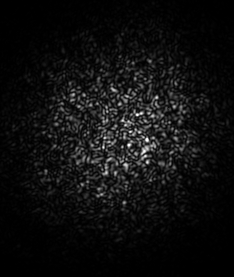
\includegraphics[width=.5\linewidth]{images/speckles_table.png}
    \caption{Image de tavelures laser. Laser Hélium-Néon diffusé sur une table de métal. Photo prise par Gabriel Genest et Prof. Daniel C. Côté, au Centre de recherche CERVO.}
    \label{fig:ex_speckles_table}
\end{figure}

\subsection{Base mathématique}
Pour bien expliquer le phénomène de tavelures, on doit s'intéresser au champs électromagnétique. Posons une onde, qu'elle soit électrique ou magnétique, sinusoïdale sous la forme phaseur:
\begin{align}
\textbf{A}(\textbf{r}) = A_0\exp{j\Phi(\textbf{r})}\label{amplitude_base}
\end{align}
où on néglige l'aspect temporel du champ électromagnétique, car il varie beaucoup plus vite que ce que le appareils peuvent mesurer et est ignorée lors des mesures. Il est suffisant de considérer un champ statique en temps. L'équation \eqref{amplitude_base} représente l'amplitude complexe des phaseurs, avec $j$ étant l'unité imaginaire telle que $j^2 = -1$ et $\Phi$ est la phase, généralement dépendante de la position $\textbf{r}$. Le modèle probabiliste des tavelures fait en sorte que $\Phi$ est une variable aléatoire continue de support $[-\pi,\pi]$, ou tout autre intervalle de longueur $2\pi$. Avec la relation d'Euler, on peut trouver une expression pour la partie réelle et celle imaginaire du champ complexe:
\begin{align}
\mathcal{R} &= A_0\cos(\Phi)\label{re_complex_amp}\\
\mathcal{I} &= A_0\sin(\Phi)\label{im_complex_amp}
\end{align}
où il est implicite que $\Phi$ dépend de la position, mais laissé de côté par soucis de concision. Il est important de noter que, sous certaines conditions générales, l'amplitude réelle $A_0$ peut être considérée aléatoire, sans changer le modèle spécifique de tavelures présenté sous peu\cite{monMemoire}.

\subsection{Tavelures pleinement développées}
Un régime intéressant de tavelures est celui où elles sont pleinement développées. Cela survient lorsque les phases sont uniformément distributées sur un intervalle de $2\pi$, généralement $[-\pi, \pi]$. Ce cas est intéressant d'un point de vue physique, car c'est celui où le déphasage est le plus aléatoire possible. Il est possible de démontrer que cette distribution maximise l'entropie, il n'y a pas de phase plus probable que les autres. Il est aussi intéressant d'un point de vue mathématique, car il simplifie beaucoup les manipulations mathématiques. On a mentionné auparavant que les tavelures surviennent lorsque plusieurs fronts d'onde s'interfèrent mutuellement. Jusqu'à présent, on a considéré un seul front d'onde (un seul phaseur). Il est alors nécessaire de développer un formalisme tenant compte de plusieurs phaseurs ayant des phases aléatoires. On écrit
\begin{align}
\textbf{A} = \frac{1}{\sqrt{N}}\sum_{k=1}^N\textbf{A}_k = \frac{1}{\sqrt{N}}\sum_{k=1}^NA_k\exp{j\Phi_k}\label{phasors_sum_base}
\end{align}
comme étant le phaseur résultant d'une somme de $N$ phaseurs. À noter ici que $\textbf{A}_k$ est le phaseur défini à l'équation \eqref{amplitude_base}. Il y a toutefois quelques conditions à propos des tavelures pleinement développées:
\begin{enumerate}
\item L'amplitude $A_k$ est indépendante de $A_m$ lorsque $k\neq m$;
\item La phase $\Phi_k$ est indépendante de $\Phi_m$ lorsque $k\neq m$;
\item Pour tout phaseur $k$, l'amplitude $A_k$ est indépendante de la phase $\Phi_k$;
\item Pour tout phaseur $k$, $\Phi_k\sim\mathcal{U}(-\pi, \pi)$.
\end{enumerate}
Ces conditions sont importante lors de la génération numérique de tavelures. On considère aussi que les amplitudes $A_k$ sont identiques et connues, elles ne sont pas aléatoires. Ce choix a peu d'impact sur la suite. Lorsque le nombre de phaseurs est grand, typiquement supérieur à $10$, on peut invoquer le théorème central limite pour trouver la distribution de la partie réelle et celle de la partie imaginaire de l'amplitude complexe résultante de l'équation \eqref{phasors_sum_base}. Les deux sont normales de moyenne nulle et de variance égale. On peut aussi montrer que ces variables aléatoires sont indépendantes.
\\ \\
On peut définir l'amplitude réelle comme étant la norme de l'amplitude complexe. Pour un grand $N$ de tavelures pleinement développées, cette amplitude réelle est distribuée selon la loi de Rayleigh. Finalement, l'intensité qu'on défini comme proportionnelle au carré de la norme de l'amplitude complexe, elle suit une distribution exponentielle lorsque $N$ est grand et les tavelures sont pleinement développées. En définissant le contraste comme
\begin{align}
C = \frac{\sigma_S}{\mu_S}\label{contraste_base}
\end{align}
où $S$ est l'intensité, on obtient que dans le cas précis des tavelures pleinement développées, le contraste est unitaire. Si la distribution de phase n'est plus $\mathcal{U}(-\pi,\pi)$, le contraste diminue. Le contraste est une quantité significative dans l'analyse de tavelures. Pour plus de détails sur le modèle de tavelures pleinement développées, se référer à \cite{monMemoire} ou encore les ouvrages de Goodman \cite{goodman_speckle_2020, goodman_statistical_2015}.
\subsection{Tavelures dans l'espace et le temps}
Les tavelures ont une certaine taille, plus ou moins bien définie, causée par la modalité d'imagerie. Selon l'instrumentation et les montages, les tavelures changent de taille. Les tavelures \textit{objectives}, donc un système non imageant, les tavelures sont de l'ordre de $1.2\frac{\lambda z}{D}$ où $\lambda$ est la longueur d'onde du laser, $z$ est la distance de propagation et $D$ est le diamètre de la région circulaire de diffusion. Pour les tavelures \textit{subjectives}, donc dans un système imageant, l'ordre de la taille est $1.2(1 + G)\lambda f_{\#}$ où $G$ est le grandissement du système et $f_{\#}$ est son \textit{f-number}. D'un point de vue expérimental, on peut aussi estimer la taille des tavelures à partir de l'autocorrélation spatiale. Cette approche est très utile pour estimer la taille des tavelures dans une image. Pour y arriver, on doit supposer une stationnarité au sens large des tavelures dans l'espace bidimensionnel. Cette condition de stationnarité n'est toutefois pas tout le temps respectée en laboratoire, notamment lorsque différents types de diffuseurs sont considérés, causant des tavelures différentes, ou lorsque les tavelures se retrouvent spatialement intégrées par les pixels. En effet, il est possible de montrer que l'existence des pixels de taille finie cause une dégradation de la qualité des images. Il est possibles que plusieurs zones indépendantes de tavelures soient superposées sur un pixel, causant une distribution d'intensité différente de l'exponentielle et par le fait même une perte de contraste.  C'est pourquoi il est néfaste d'avoir des tavelures trop petite comparativement à la taille des pixels physiques. On recommande au moins de pixels de large pour les tavelures\cite{kirkpatrick_detrimental_2008}. De cette manière, un pixel unique ne devrait qu'avoir une seule région de corrélation spatiale, en général, et limiter la perte de contraste. L'importance du contraste se fera plus évidente lorsque les variabilités temporelles des tavelures seront présentées.
\\ \\
Le mouvement aléatoire ou ordonné des diffuseurs causent une variation temporelle des tavelures. Dans le cas aléatoire, il peut s'agir de mouvement brownien ou de vibrations ambiantes. Dans le cas ordonné, il peut s'agir d'un écoulement ou d'un flot. Si on filme des tavelures dans de telles circonstances, elles apparaîtront et disparaîtront dans le temps. On peut ainsi calculer une décorrélation temporelle des tavelures qui peut révéler de l'information importante. Dans un premier temps, il y a le temps caractéristique de décorrélation. Cette quantité indique à quel point les diffuseurs bougent rapidement. Plus le temps caractéristique est élevé, plus les tavelures sont stables. Dans un second temps, il existe des modèles reliant le temps caractéristique à d'autres propriétés, comme la visco-élasticité\cite{hajjarian_evaluating_2012}. Obtenir le temps caractéristique n'est pas nécessairement évident. Les démarches changent selon l'ergodicité ou la stationarité des tavelures\cite{zheng_direct_2022}. De plus, obtenir une approche précise, de l'ordre du pixel ou d'un petit regroupement de pixels, peut devenir assez long et demander des corrections non triviales\cite{zheng_correcting_2022}.
\\ \\
La décorrélation temporelle des tavelures entraîne une toute autre problématique en lien avec les statistiques spatiale. Une caméra ou un capteur quelconque ne produit pas une image instantannément. Il est nécessaire d'imager sur un certain délai pour capter les photons émis et produire une image bien définie. Ce délai est appelé temps d'acquisition ou temps d'intégration. On peut voir cette période comme l'intégration d'une infinité de motifs de tavelures instantannés. Selon le temps caractéristique, ces motifs peuvent être fortement ou faiblement corrélés. Dans le cas où l'intégration sur fait sur une séquence faiblement corrélée, par exemple le temps d'intégration est beaucoup plus petit que le temps caractéristique, on intègre sur un motif assez stable, donc n'entraînant pas de problèmes significatifs avec le contraste. Par contre, dans le cas contraire où le temps d'intégration est beaucoup plus grand que le temps caractéristique, on intègre sur plusieur un motif variant rapidement, donc entraînant une perte de contraste, tel que montré à la figure \ref{fig:contrastFctT_tauc}, tirée de \cite{monMemoire}.
\begin{figure}[h!!]
    \centering
    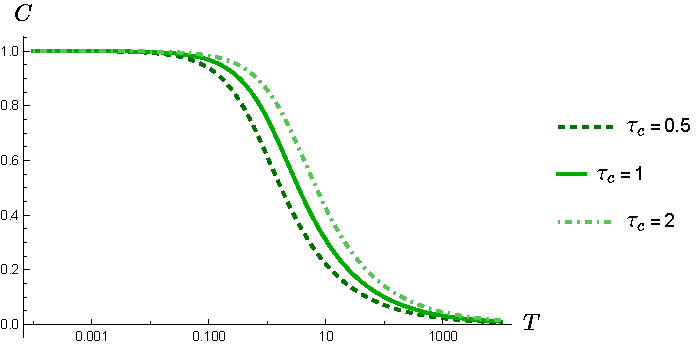
\includegraphics[width=1\linewidth]{images/exponCorrDiffTauC.pdf}
    \caption{Contraste spatial théorique d'une image de tavelure ayant une autocorrélation temporelle exponentielle pour divers temps caractéristiques $\tau_c$ en fonction du temps d'acquisition $T$. Les unités de temps sont arbitraires.}
    \label{fig:contrastFctT_tauc}
\end{figure}
\newpage
\section{Création du jeu de données}



































\printbibliography
\end{document}
